%%%%%%%%%%%%%%%%%%%%%%%%%%%%%%%%%%%%%%%%%
% FRI Data Science_report LaTeX Template
% Version 1.0 (28/1/2020)
% 
% Jure Demšar (jure.demsar@fri.uni-lj.si)
%
% Based on MicromouseSymp article template by:
% Mathias Legrand (legrand.mathias@gmail.com) 
% With extensive modifications by:
% Antonio Valente (antonio.luis.valente@gmail.com)
%
% License:
% CC BY-NC-SA 3.0 (http://creativecommons.org/licenses/by-nc-sa/3.0/)
%
%%%%%%%%%%%%%%%%%%%%%%%%%%%%%%%%%%%%%%%%%

\documentclass[fleqn,moreauthors,10pt]{ds_report}
\usepackage[english]{babel}
\graphicspath{{fig/}}
\usepackage{stix}
\definecolor{delim}{RGB}{20,105,176}
\lstdefinelanguage{json}{
    basicstyle=\scriptsize\ttfamily,
    numbers=left,
    numberstyle=\scriptsize,
    stepnumber=1,
    numbersep=8pt,
    showstringspaces=false,
    breaklines=true,
    frame=lines
}
\usepackage{mathtools}
\JournalInfo{FRI Data Science Project Competition 2025}
\Archive{Final report} 
\PaperTitle{Classifying companies by industry} 
\Authors{Jernej Avsec and Luka Bajić}
\affiliation{\textit{Advisors: Prof. Erik Štrumbelj}}
\Keywords{predictive machine learning, taxonomy/hierarchy classification, natural language processing}
\newcommand{\keywordname}{Keywords}

%----------------------------------------------------------------------------------------
%	ABSTRACT
%----------------------------------------------------------------------------------------

\Abstract{
The North American Industry Classification system is a standard for classifying companies. Unfortunately, the classification is readily available only for a small number of companies. We address this problem by developing an approach that can classify any company using a predetermined set of information about that company. Our approach is based on hierarchical prompting of a general-purpose LLM with company information and classification code descriptions. Using real-world data provided by PredictLeads, we demonstrate operationally acceptable performance for 6-digit codes and near-perfect performance for shorter codes. We also demonstrate how the approach can be scaled by training a secondary classifier. The scalable approach is currently below operationally acceptable performance, but is cost-effective and with a lot of potential for improvement.}

%----------------------------------------------------------------------------------------

\begin{document}

% Makes all text pages the same height
\flushbottom 

% Print the title and abstract box
\maketitle 

% Removes page numbering from the first page
\thispagestyle{empty} 

%----------------------------------------------------------------------------------------
%	ARTICLE CONTENTS
%----------------------------------------------------------------------------------------

\section*{Introduction}

The North American Industry Classification System (NAICS) is a popular standard for classifying companies that is used by US federal statistical agencies and many other entities. The current NAICS 2022 code (\url{https://www.naics.com/search/}) is a 6-digit code composed out of sector, subsector, industry group, NAICS industry, and national industry (US, Canada, and Mexico-specific sub-classifications of the industry).

To illustrate the NAICS classification, here are two examples of how the code is broken down. The first is for \emph{MGM Holdings Inc.} (512110): 
\begin{small}
\begin{align*}
&\text{51 - Information}\\
&\text{5121 - Motion Picture and Video Industries}\\
&\text{512110 - Motion Picture and Video Production} 
\end{align*}
\end{small}
\noindent and the second one for the \textit{Coca Cola Company} (311930)
\begin{small}
\begin{align*}
&\text{31 - Manufacturing}\\
&\text{3119 - Other Food Manufacturing}\\
&\text{311930 - Flavoring Syrup and Concentrate Manufacturing} 
\end{align*}
\end{small}

We can see that NAICS is a hierarchical classification. It currently consists of 1,012 active codes. A company is typically assigned one code, but it is not uncommon for more than one code to be applicable to the same company. For example, Soft Drink Manufacturing (312111) is also a reasonable code for the Coca Cola Company.


Our research is motivated by the practical problem of PredictLeads, who would like to provide their customers with NAICS codes for the millions of companies that they keep track of. NAICS codes are currently publicly available only for a handful of companies and almost exclusively for companies from North America. In principle, classifications could be obtained from third-party providers, such as the NAICS Association. In practice, however, this is not possible. First, the cost would be prohibitive. And second, as we demonstrate later, the quality of data from third-party providers is questionable, which also limits the availability of a ground truth dataset. Furthermore, NAICS codes are revised every 5 years. For these reasons, the most reasonable approach is to automate the prediction of NAICS codes from more readily available company information.

In the remainder of the report we first describe the real-world data provided by PredictLeads. Then we describe our initial investigation of the validity of third-party NAICS classifications and the variability of NAICS classifications across different human raters. This allowed us to establish that there is no single-source ground truth for NAICS classifications and that a large labeled dataset is infeasible. Instead, we utilize general-purpose LLMs to provide NAICS codes using company information and code descriptions. Our approach is a combination of refined prompting strategies, careful data pre-processing, and taking advantage of the hierarchical structure of the NAICS code.

We demonstrate how our approach can be used to predict very accurate NAICS codes on real-world data and exceed the operationally acceptable classification performance (+95\% at-least-one-match accuracy for 6-digit codes). However, we also consider the special, but practically relevant case where the number of companies to be classified is so large that the use of a general-purpose LLM is cost-prohibitive. For scalability, we propose generating a sufficiently large labeled dataset, which is then used to train a classifier. This approach, using pre-trained text embeddings, currently leads to below operationally acceptable performance, but is cost-effective and has a lot of potential for improvement by fine-tuning for this particular classification task.

\section*{Data}

We used several different datasets in our work. In this section we describe them and give them easily identifiable names that we will reference in the methods and experiments.

First, we collected all information about the NAICS 2022 classification from the official source (\url{https://www.naics.com/six-digit-naics}). These include code descriptions, example companies, explanations of how to apply the code, cross references, and index entries, all for 2-through-6 digit codes.

\subsection*{Company information - high-quality 32k dataset}

PredictLeads provided us with a company information dataset from their real-world data, consisting of approximately 32k companies with high-quality textual and meta-data. The data include LinkedIn data (decription, slogan) and company website data (domain, description, job openints, etc.). We construct our initial \textbf{Test set A} by randomly sampling with replacement 100 companies from those listed on the NAICS website (official NAICS code and PredictLeads company data are avaiable) and 100 companies from the 32k dataset (official NAICS code not avaiable).

\subsection*{Ground truth and inter-rater variability}

An initial review of official NAICS codes revealed outdated and invalid codes that had to be removed. This called into question the reliability of what was initially thought of as the gold-standard ground truth. To further investigate the difficulty of the NAICS classification problem, we asked 3 human annotators (PredictLeads, one of the authors, and an external annotator) to provide codes for Test set A. Combined with official NAICS labels, we thus obtained 4 separate ground truth annotations.

The inter-rater agreement rates in Figure \ref{fig:interrater} show relatively low agreement between human raters even on the the 2-digit code. Note that rater 3 performed the annotation only by correcting the existing official codes, where necessary, resulting in higher agreement with official codes.

\begin{figure}
    \centering
    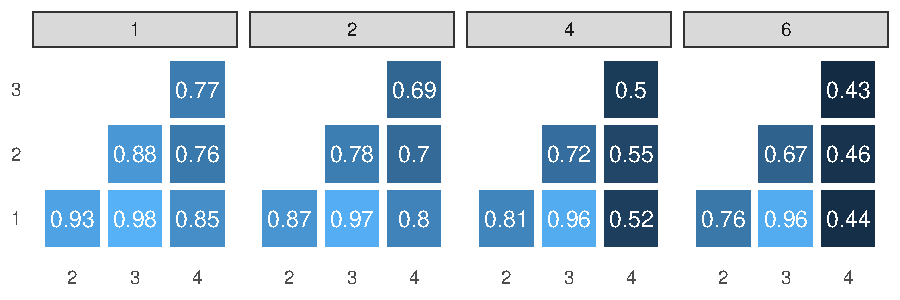
\includegraphics[width=\linewidth]{fig/interrater.pdf}
    \caption{Proportion of cases where at least one code was common to both raters for Test set A. Results are broken down by number of digits considered (1, 2, 4, and 6, the complete code). Note that rater 1 are offical NAICS codes.}
    \label{fig:interrater}
\end{figure}

\subsection*{Company information - representative 100k dataset}

After we developed our methodology, we requested an additional sample of 100k companies to use as a training set for scalability and a final validation of our approach. Unlike the initial sample, this was a representative sample from the target population of 40M companies that PredictLeads would be interested in making a prediction for.

The only practical constraint is that the sample contains at least 100 characters of textual description. Most fields can now be empty and the overall quality of the data is expected to be lower than the initial 32k dataset. Figure \ref{fig:distribution} also shows how the distribution of NAICS codes changes when moving from mostly top companies to a more general population of companies. Most evident is less manufacturing and more retail and services companies.

We again set aside 200 companies chosen at random with replacement to serve as a final test set (\textbf{Test set B}).

\begin{figure}[ht]\centering
	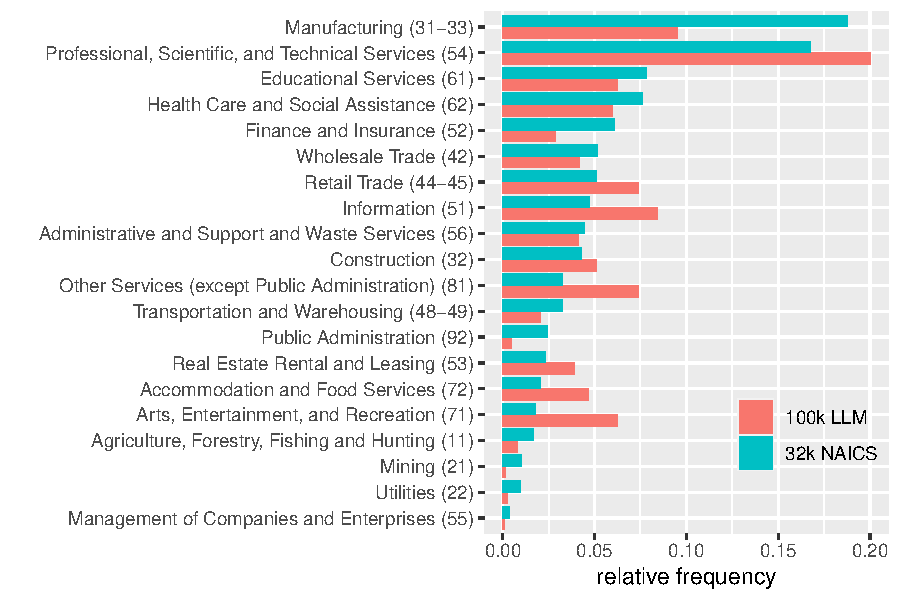
\includegraphics[width=\linewidth]{fig/distribution.pdf}
	\caption{A comparison of 2-digit NAICS code relative frequencies on the 32k dataset (official NAICS codes) and the 100k dataset (labeled by our best performing Gemini-H (see Methods and Results)).}
	\label{fig:distribution}
\end{figure}


\section*{Methods}

\subsection*{Classifying NAICS codes with LLMs}

We used two general-purpose LLMs: Gemini 2.0-flash (henceforth \textbf{Gemini}) and GPT-4o-mini (\textbf{GPT}). In our initial experiments we also considered DeepSeek's deepseek-chat, but eventually gave up because of lag and availability issues.

All models considered receive both company specific information and a set of candidate NAICS codes. Company information includes website meta-data, high and low priority keywords, LinkedIn slogan, LinkedIn description, and LinkedIn industry classification. The prompt also included the following general instructions:

\begin{small}
\begin{enumerate}
\item Classify the company's main webpage content into relevant NAICS codes (\{N\}) digits).
\item Only select NAICS codes that are directly relevant to the company's activities.
\item Sort the NAICS codes from most relevant to least relevant.
\item Return the results in a structured JSON format.
\item Consider the primary business activities, not peripheral or secondary services.
\item Include "confidence\_score", that indicates confidence in the classification.
 \item There must be at least one NAICS code chosen.
\end{enumerate} 
\end{small}

\noindent and an example JSON output with code and confidence score.

The first improvement over this base model was the inclusion of NAICS code names (models marked with \textbf{C}), rather than relying solely on the LLM’s prelearned knowledge about the codes (as described in the NAICS 2022 classification section)

The second improvement is to take advantage of the the hierarchical nature of the NAICS code. These models only consider the subset of codes corresponding to predictions made at the preceding level. That is, first classify the first two digits, where accuracy is generally higher, then move onto the next 2, and finally the complete 6-digit code. Hierarchical models use either only code names and descriptions as context (H), or all available scraped information about the codes (HE).

Finally, we use confidence score thresholding to improve absolute accuracy. That is, low confidence predictions are discarded. We construct calibration curves by grouping predicted label-confidence pairs into quantile-based bins and comparing predicted confidence with observed accuracy. For each bin, we compute the average predicted probability, the observed fraction of correct predictions, and the standard error.

\subsection*{Classifying LLM output for scalability}

For this purpose we utilize pre-trained ModernBERT \cite{modernbert} and 3 different classification models. We train them on 100k labeled samples (excluding Test set B) obtained with the Gemini model. We set aside, at random, 90k companies for training and 10k for validating. Note that for labeling we keep the most probable code and all codes with probability $> 0.85$. We used three classifiers:
\begin{itemize}
    \item \textbf{Logistic Regression (LogisticReg)}: a single linear layer with dropout (0.1) applied after a $\tanh$ nonlinearity, following the BERT pooler convention.
    \item \textbf{Two-layer MLP (MLPHead)}: applies $\tanh$ to the input, followed by two linear layers with ReLU activation and dropout (0.3), projecting through a hidden layer of size 256.
    \item \textbf{Three-layer MLP (MLPHead3Layer)}: extends the MLPHead by adding an additional hidden layer (sizes: 512 and 256), with ReLU and dropout (0.2) after each layer. 
\end{itemize}

Each model is trained on modernBERT \cite{modernbert} encoded company information that includes website meta-data, high and low priority keywords, LinkedIn slogan, LinkedIn description, and LinkedIn industry classification. Because of unbalanced labels, we used sigmoid focal loss for optimization. 

The biggest obstacle in this approach is the amount of rare codes in the Gemini-generated 100k training set, which is not only a property of this dataset, but of NAICS codes in general (see Figure \ref{fig:distribution}). We try to combat this issue with regularization during fine-tuning and obtain results shown in Table \ref{tab:bert}. We also omit all codes with frequency less than two, which cannot be used in both training and test set, so we are left with 957 classes. 

\subsection*{Evaluation metrics}

We prompt all models to output at least one code per company, as well as a confidence score for each code. We do not specify an upper bound on the number of codes, so we evaluate the results in two ways:

\begin{itemize}
    \item \textbf{At-least-one-match accuracy (CA)} - the model returned at least one code that is present in at least one of the ground truth sources. This can be viewed as classification accuracy, albeit with more than one attempt.
    \item \textbf{Absolute accuracy (ABS)} - ratio between correct codes and the total number of returned codes.
\end{itemize}

Note that a numbered suffix tells us what part of the code the metric is limited to. For example, CA-2 is the at-least-one-match accuracy for the fist two digits of the code.

LLMs in sometimes return invalid or outdated codes. Since there is no training involved, we see no benefit in penalizing invalid codes. We implement a function for mapping outdated codes (i.e. from 2017 and 2012 NAICS standards) into 2022 codes according to official NAICS documentation.

Due to a lack of a gold-standard ground-truth (see Ground truth and inter-rater variability), it is common that a LLM output code is valid, but is not in any ground-truth set. For each of the two 200-company test sets, after achieving sufficiently good performance with the LLMs, we also added a ground-truth based on manually validated LLM output codes.

\section*{Results}

Table \ref{tab:results1} shows a comparison of the models on Test set A. Even without a context, GPT performs reasonably well. However, best performance is achieved with context and hierarchical prompting. The hierarchical approach substantially improves classification performance. The improvement is biggest for the longer codes, as we would expect, and brings performance to an operationally acceptable level. As shown in Figure \ref{fig:absolute}, the hierarchical approach also substantially improves absolute accuracy. And, most notably, the best models classification performance does not drop by much when applied to the representative Test set B (see \ref{tab:bert_test})!

\begin{table}[tbp]
\centering
\resizebox{1.0 \linewidth}{!}{\begin{tabular}{l c c c c c c c c}
\hline
Model & CA-1 & CA-2 & CA-3 & CA-4 & CA-5 & CA-6 & ABS-6 & avg \# codes \\ \hline
GPT  & 0.964 & 0.938 & 0.923 & 0.872 & 0.836 & 0.805 & 0.442 & 2.89  \\
GPT-C  & 0.969 & 0.933 & 0.923 & 0.856 & 0.846 & 0.795 & 0.283 & 3.07   \\
Gemin  & 0.969 & 0.969 & 0.954 & 0.938 & 0.897 & 0.862 & 0.510 & 2.99 \\
Gemini-C  & \textbf{1.000} & \textbf{1.000} & \textbf{0.995} & 0.979 & 0.979 & 0.974 & 0.549 & 3.33 \\
Gemini-H   & 0.985 & 0.985 & 0.979 & 0.944 & 0.938 & 0.933 & 0.571 & 2.91 \\
Gemini-HE  & \textbf{1.000} & \textbf{1.000} & \textbf{0.995} & \textbf{0.990} & \textbf{0.985} & \textbf{0.979} & \textbf{0.687} & 2.75 \\
\hline
\end{tabular}}
\caption{Model comparison on Test set A. The average number of codes per company is included. Note that all the differences between the best performing model (in bold) and the second best are more than 2 standard errors. While the test set is relatively small, the accuracies close to 100\% have small variance.}
\label{tab:results1}
\end{table}

\begin{figure}[tbp]\centering
	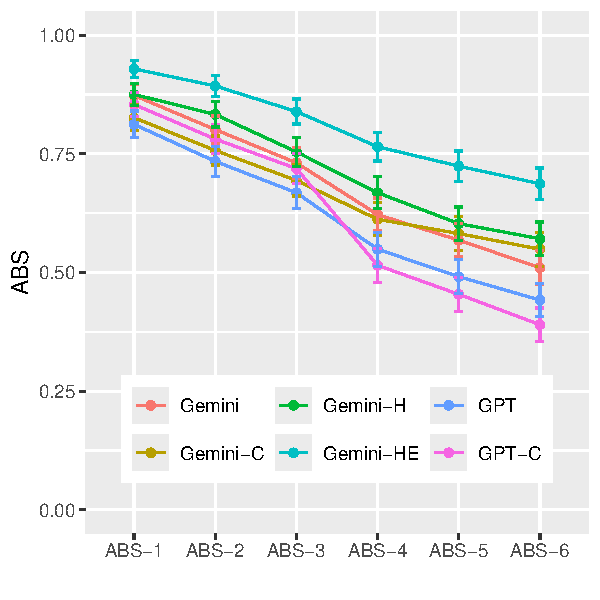
\includegraphics[width=0.7\linewidth]{abs.pdf}
	\caption{Absolute accuracy comparison on Test set A, comparing all models featured so far. Error bars are one standard error.}
	\label{fig:absolute}
\end{figure}

\subsection*{Scalability}

The performance of predicting the codes output by our best general-purpose LLM-based model is shown in Table \ref{tab:bert}. Predicted codes from classifier were chosen with condition of at least one code, and all the rest that have probability $>0.3$. Performance is relatively poor and, as we would expect, translates into poor test performance on Test set B in Table \ref{tab:bert_test}. However, if classification performance can be improved by fine-tuning for this task, the results are encouraging in terms of resources required. The bottleneck, computing ModernBERT embeddings, took 40 minutes for 100,000 examples (consumer laptop with GPU NVidia RTX 2060 with 6GB). This translates to about 2 weeks for 40M companies.

\begin{table}[htb]
\centering
\resizebox{1.0 \linewidth}{!}{\begin{tabular}{l c c c c c c c c}
\hline
Model & CA-1 & CA-2 & CA-3 & CA-4 & CA-5 & CA-6 & ABS-6 & avg \# codes \\ \hline
Log. Reg.  & 0.667 & 0.571 & 0.532 & 0.452 & 0.428 & 0.410 & 0.398 & 1.06  \\
2-layer NN & 0.681 & 0.586 & 0.547 & 0.472 & 0.450 & 0.432 & 0.395 & 1.18   \\
3-layer NN & 0.699 & 0.609 & 0.567 & 0.492 & 0.467 & 0.451 & 0.414 & 1.18 \\

\hline
\end{tabular}}
\caption{An evaluation of the classifiers ability to predict codes output by the best LLM.}
\label{tab:bert}
\end{table}



\begin{table}[!htb]
\centering
\resizebox{1.0 \linewidth}{!}{\begin{tabular}{l c c c c c c c c}
\hline
Model & CA-1 & CA-2 & CA-3 & CA-4 & CA-5 & CA-6 & ABS-6 & avg \# codes \\ \hline
Gemini-HE  & 0.955 & 0.940 & 0.930 & 0.930 & 0.925 & 0.925 & 0.685 & 2.22 \\
Log. Reg.  & 0.325 & 0.130 & 0.105 & 0.035 & 0.035 & 0.030 & 0.025 & 1.21  \\
2-layer NN & 0.380 & 0.165 & 0.140 & 0.050 & 0.040 & 0.030 & 0.020 & 1.50   \\
3-layer NN & 0.315 & 0.130 & 0.120 & 0.045 & 0.035 & 0.035 & 0.028 & 1.43 \\

\hline
\end{tabular}}
\caption{Comparison of best LLM and classification models on Test set B.}
\label{tab:bert_test}
\end{table}

%------------------------------------------------

\section*{Conclusion}

We demonstrate that it is possible to achieve operationally acceptable NAICS code classification performance using general-purpose LLMs. While decent performance can be achieved with a relatively simple prompt, we made key improvements by including code description context, hierarchical prompting, and confidence score thresholding. The latter two improvements are particularly important for high absolute code accuracy, as opposed to just high at-least-one-match accuracy.

For a scalable solution we propose generating a labeled training set to learn a less resource-intensive specialized classifier. Our initial approach with ModernBERT embeddings did not give satisfactory results, but has a lot of potential for improvement. In particular, we did not yet attempt fine-tuning ModernBERT (or parts of it) to our particular classification task, due to time and resource constraints. This is the most important direction for future work.

Another notable challenge are rare codes. Some NAICS codes are so rare that they only appear once or twice for every 100k companies, if at all. The general-purpose approach should in principle be able to predict those codes, but training a classifier requires us to have the code in the training set. This implies the need for stratified sampling, however, companies have to be labeled, which would require a larger training set and would be more costly. And in both cases our evaluation was focused on \emph{on average} performance. The performance on rare codes, if those were an operational priority, is not well understood and cannot be well understood without extensive manual validation.

%------------------------------------------------

\section*{Acknowledgments}

We would like to thank PredictLeads for their data and for entrusting us to work on their problem, in particular Anže Glušič for providing an excellent starting point for LLM-based classification. We would also like to thank Urška Žnidarič for her NAICS classification.

%----------------------------------------------------------------------------------------
%	REFERENCE LIST
%----------------------------------------------------------------------------------------
\bibliographystyle{unsrt}
\bibliography{bibliography}


\end{document}